\section{Proof of quasi-determinism for $\lambdaLVish$}\label{s:quasi-proof-of-quasi-determinism}

In this section, \either{I}{we} give a proof of quasi-determinism for
$\lambdaLVish$ that formalizes the claim made earlier in this \either{chapter}{section}:
that, for a given program, although some executions may raise
exceptions, all executions that produce a final result will produce
the same final result.

The quasi-determinism theorem \either{I}{we} show says that if two executions
starting from a configuration $\conf$ terminate in configurations
$\conf'$ and $\conf''$, then either $\conf'$ and $\conf''$ are the
same configuration (up to a permutation on locations), or one of them
is $\error$.  As with the determinism proof for $\lambdaLVar$
in Section~\ref{s:lvars-proof}, quasi-determinism follows from a
series of supporting lemmas.  The basic structure of the proof follows
that of the $\lambdaLVar$ determinism proof closely.  However, instead
of the Independence property that \either{I}{we} showed for $\lambdaLVar$
(Lemma~\ref{lem:lvars-independence}), here \either{I}{we} prove a more general property,
Generalized Independence (Lemma~\ref{lem:generalized-independence}),
that accounts for the presence of both freezing and arbitrary update
operations in $\lambdaLVish$.  Also, in the setting of $\lambdaLVish$,
the Strong Local Confluence property
(Lemma~\ref{lem:lvars-strong-local-confluence}) becomes Strong Local
\emph{Quasi-}Confluence
(Lemma~\ref{lem:strong-local-quasi-confluence}), which allows the
possibility of an $\error$ result, and the quasi-confluence lemmas
that follow---Strong One-sided Quasi-Confluence
(Lemma~\ref{lem:strong-one-sided-quasi-confluence}), Strong
Quasi-Confluence (Lemma~\ref{lem:lvars-strong-confluence}), and
Quasi-Confluence (Lemma~\ref{lem:lvars-confluence})---all follow this
pattern as well.
\ifdefined\JOURNAL
We give only the statements of the quasi-determinism theorem and its
supporting lemmas here; their proofs appear
in~\cite{lvars-dissertation}.
\fi

\subsection{Permutations and permutability}\label{subsection:quasi-permutations}

As with $\lambdaLVar$, the $\lambdaLVish$ language is nondeterministic with
respect to the names of locations it allocates.  We therefore prove
quasi-determinism up to a permutation on locations.  We can reuse the
definition of a permutation verbatim from
Section~\ref{subsection:lvars-permutations}:

\DefPermutation

We can lift $\pi$ to apply expressions, stores, and
configurations.
\ifdefined\DISSERTATION
Because expressions and stores are defined slightly
differently in $\lambdaLVish$ than they are in $\lambdaLVar$, we must
update our definitions of permutation of a store and permutation of an
expression:

\DefPermutationExpression

\DefPermutationStore

And the definition of permutation of a configuration is as it was before:

\DefPermutationConfiguration
\fi
We can then prove a Permutability lemma for $\lambdaLVish$, which says
that a configuration $\conf$ can step to $\conf'$ exactly when
$\pi(\conf)$ can step to $\pi(\conf')$.

\LemPermutability
\ifdefined\DISSERTATION
\begin{proof}
  Similar to the proof of Lemma~\ref{lem:lvars-permutability}
  (Permutability for $\lambdaLVar$); see
  Section~\ref{section:permutability-proof}.
\end{proof}
\fi

\subsection{Internal Determinism}

In \either{Chapter}{Section}~\ref{ch:lvars}, we saw that the reduction
semantics for $\lambdaLVar$ is internally deterministic: that is, if a
configuration can step by the reduction semantics, there is only one
rule by which it can step, and only one configuration to which it can
step, modulo location names.  For $\lambdaLVish$, we can also show an
internal determinism property, but with a slight additional wrinkle.

In $\lambdaLVish$, the {\sc E-Spawn-Handler} rule picks out an
eligible element $d_2$ from the set $Q$ (that is, an event) and
launches a new callback thread to handle that event.  But, since there
could be more than one eligible element in $Q$ that {\sc
  E-Spawn-Handler} could choose, the choice of event is a source of
nondeterminism.  Therefore, we show that $\lambdaLVish$ is internally
deterministic modulo \emph{choice of events}, as well as modulo
location names.  This property will be useful to us later on in the
proof of Strong Local Quasi-Confluence
(Lemma~\ref{lem:strong-local-quasi-confluence}).

\LemInternalDeterminism
\ifdefined\DISSERTATION
\begin{proof}
  Straightforward by cases on the rule of the reduction semantics by
  which $\conf$ steps to $\conf'$; the only interesting case is for
  the {\sc E-New} rule.  See
  Section~\ref{section:internal-determinism-proof}.
\end{proof}
\fi

\subsection{Locality}

Just as with the determinism proof for $\lambdaLVar$, proving
quasi-determinism for $\lambdaLVish$ will require us to handle
expressions that can decompose into redex and context in multiple
ways.  An expression $e$ such that $e = \evalctxt{E_1}{e_1} =
\evalctxt{E_2}{e_2}$ can step in two different ways by the {\sc
  E-Eval-Ctxt} rule: $\config{S}{\evalctxt{E_1}{e_1}} \ctxstepsto
\config{S_1}{\evalctxt{E_1}{e'_1}}$, and
$\config{S}{\evalctxt{E_2}{e_2}} \ctxstepsto
\config{S_2}{\evalctxt{E_2}{e'_2}}$.

The Locality lemma says that the $\ctxstepsto$ relation acts
``locally'' in each of these steps. The statement of the Locality
lemma is the same as that of Lemma~\ref{lem:lvars-locality} (Locality
for $\lambdaLVar$), but the proof must account for the set of possible
evaluation contexts in $\lambdaLVish$ being different (and larger)
than the set of evaluation contexts in $\lambdaLVar$.

\LemLocality
\ifdefined\DISSERTATION
\begin{proof}
  Let $e = \evalctxt{E_1}{e_1} = \evalctxt{E_2}{e_2}$.  The proof is
  by induction on the structure of the expression $e$.  See
  Section~\ref{section:locality-proof}.
\end{proof}
\fi

\subsection{Monotonicity}\label{subsection:quasi-monotonicity}

The Monotonicity lemma says that, as evaluation proceeds according to
the $\parstepsto$ relation, the store can only grow with respect to
the $\leqstore{}{}$ ordering.

\LemMonotonicity
\ifdefined\DISSERTATION
\begin{proof}
  Straightforward by cases on the rule of the reduction semantics by
  which $\config{S}{e}$ steps to $\config{S'}{e'}$. The interesting
  cases are for the {\sc E-New} and {\sc E-Put} rules.  See
  Section~\ref{section:monotonicity-proof}.
\end{proof}
\fi

\subsection{Generalized Independence}\label{subsection:quasi-generalized-independence}

Recall from \either{Chapter}{Section}~\ref{ch:lvars} that in order to prove determinism
for $\lambdaLVar$, we needed to establish a ``frame property'' that
captures the idea that independent effects commute with each other.
For $\lambdaLVar$, the Independence lemma
(Lemma~\ref{lem:lvars-independence}) established that property.  It
shows that, if a configuration $\config{S}{e}$ can step to
$\config{S'}{e'}$, then it is possible to ``frame on'' an additional
store $S''$ without interfering with the ability to take a step---that
is, $\config{\lubstore{S}{S''}}{e} \parstepsto
\config{\lubstore{S'}{S''}}{e'}$, subject to certain restrictions on
$S''$.

For $\lambdaLVish$, we need to establish a similar frame property.
However, since we have generalized from @put@ to $\PUTi$, we also
need to generalize our frame property.  In fact, the original
Lemma~\ref{lem:lvars-independence} does not hold for $\lambdaLVish$.
As an example, consider an LVar whose states form a lattice
$\bot < 0 < 1 < \top$.  Consider the transition
\[
\config{\store{\storebinding{l}{0}{\frozenfalse}}}{\putiexp{l}}
\parstepsto \config{\store{\storebinding{l}{1}{\frozenfalse}}}{\unit},
\]
where the update operation $u_i$ happens to increment its argument by
one.  Now suppose that we wish to ``frame'' the store
$\store{\storebinding{l}{1}{\frozenfalse}}$ onto this transition using
Lemma~\ref{lem:lvars-independence}; that is, we wish to show that
\[
\config{\lubstore{\store{\storebinding{l}{0}{\frozenfalse}}}{\store{\storebinding{l}{1}{\frozenfalse}}}}{\putiexp{l}}
\parstepsto
\config{\lubstore{\store{\storebinding{l}{1}{\frozenfalse}}}{\store{\storebinding{l}{1}{\frozenfalse}}}}{\unit}.
\]
We know that
$\lubstore{\store{\storebinding{l}{1}{\frozenfalse}}}{\store{\storebinding{l}{1}{\frozenfalse}}}
\neq \topS$, which is required to be able to apply
Lemma~\ref{lem:lvars-independence}.  Furthermore,
$\store{\storebinding{l}{1}{\frozenfalse}}$ is non-conflicting with
the original transition, since no new locations are allocated between
$\store{\storebinding{l}{0}{\frozenfalse}}$ and
$\store{\storebinding{l}{1}{\frozenfalse}}$.  But it is \emph{not} the
case that
$\config{\lubstore{\store{\storebinding{l}{0}{\frozenfalse}}}{\store{\storebinding{l}{1}{\frozenfalse}}}}{\putiexp{l}}$
steps to
$\config{\lubstore{\store{\storebinding{l}{1}{\frozenfalse}}}{\store{\storebinding{l}{1}{\frozenfalse}}}}{\unit}$,
since $u_{p_i}((\lubstore{S}{S''})(l)) = \topp$.  (As before,
$u_{p_i}$ is the update operation $u_i$, lifted from lattice elements
$d$ to states $\state{d}{\status}$.)

What went wrong here?  The problem is that, as previously discussed in
Section~\either{\ref{subsection:lvars-generalizing-from-least-upper-bound-writes}}{\ref{s:lvars-generalizing}},
lub operations do not necessarily commute with arbitrary update
operations.  In $\lambdaLVar$, where the only ``update operation'' is
a lub write performed via @put@, it is fine that the Independence
lemma uses a lub operation to frame $S''$ onto the transition. For
$\lambdaLVish$, though, we need to state our frame property in a way
that will allow it to accommodate any update operation from the given
set $U$.

Therefore, \either{I}{we} define a \emph{store update operation} $U_S$ to be a
function from stores to stores that can add new bindings, update the
contents of existing locations using operations $u_i$ from the given
set $U$ of update operations (or, more specifically, their lifted
versions $u_{p_i}$), or freeze the contents of existing locations.

\DefStoreUpdateOperation

\noindent Definition~\ref{def:store-update-operation} says that applying $U_S$
to $S$ either updates (using some $u_{p_i} \in U_p$) or freezes the
contents of each $l \in \dom{S}$.  Since the identity function is
always implicitly a member of $U_p$, $U_S$ can act as the identity on
the contents of locations.  $U_S$ can also add new bindings to the
store it operates on; however, it cannot change existing location
names.

With Definition~\ref{def:store-update-operation} in hand, we can state
a more general version of the Independence lemma:

\LemGeneralizedIndependence
\ifdefined\DISSERTATION
\begin{proof}
  By cases on the rule of the reduction semantics by which
  $\config{S}{e}$ steps to $\config{S'}{e'}$.  The interesting cases
  are for the {\sc E-New}, {\sc E-Put}, {\sc E-Freeze-Final}, and {\sc
    E-Freeze-Simple} rules.  See
  Section~\ref{section:generalized-independence-proof}.
\end{proof}
\fi

Lemma~\ref{lem:generalized-independence} has three preconditions on
the store update operation $U_S$, two of which mirror the two
preconditions on $S''$ from the original Independence lemma: the
requirement that $U_S(S') \neq \topS$, and the requirement that $U_S$
is non-conflicting with the transition from $\config{S}{e}$ to
$\config{S'}{e'}$.
Definition~\ref{def:non-conflicting-store-update-operation} revises
our previous definition of ``non-conflicting'' to apply to store update
operations.  It says that $U_S$ is non-conflicting with the transition
$\config{S}{e} \parstepsto \config{S'}{e'}$ if, for all locations
allocated in the transition, $U_S$ does not interfere with those
locations.  For instance, if $l$ is allocated in the transition from
$\config{S}{e}$ to $\config{S'}{e'}$, then $l \notin \dom{U_S(S)}$
(that is, $U_S$ cannot add a binding at $l$ to $S$), and $(U_S(S'))(l)
= S'(l)$ (that is, $U_S$ cannot update the contents of $l$ in $S'$).

\DefNonConflictingStoreUpdateOperation

\ifdefined\DISSERTATION
\begin{wrapfigure}{r}{2in}
\vspace{-1.5em}
\begin{center}
  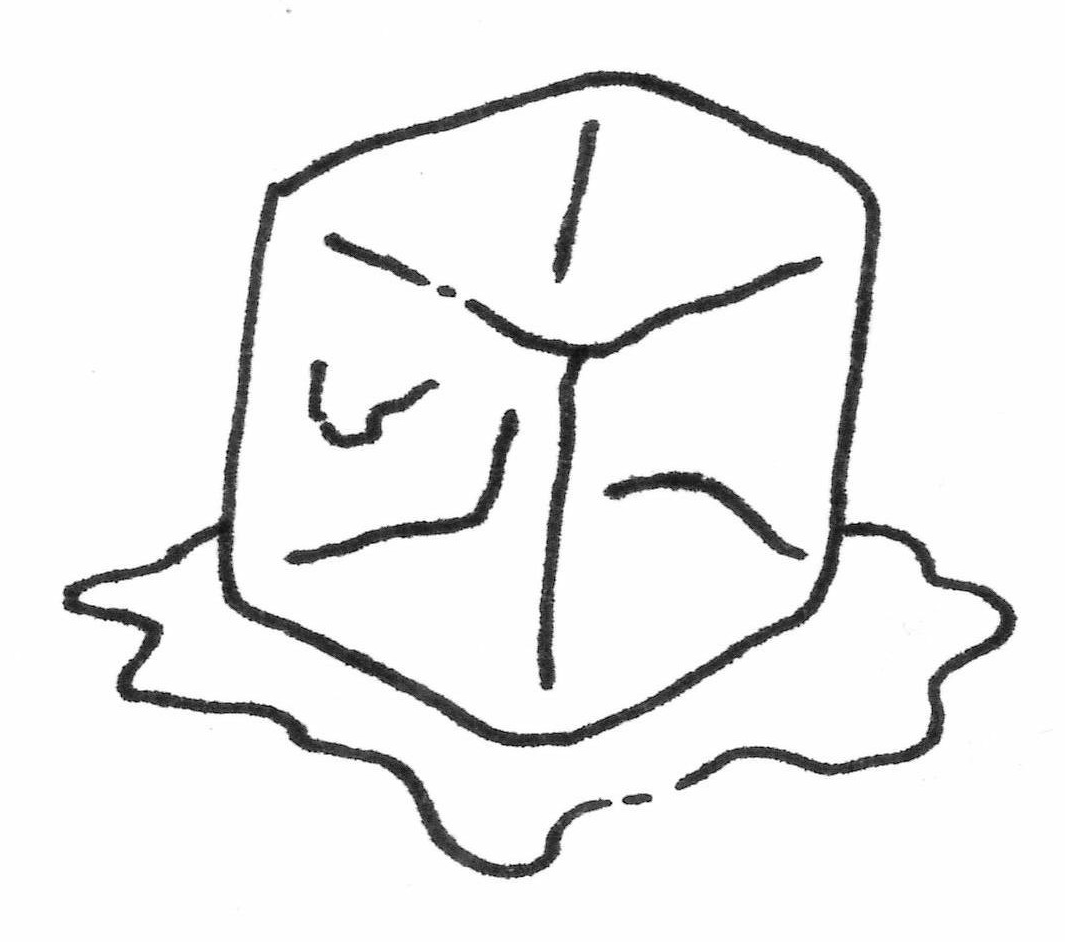
\includegraphics[scale=0.13]{../illustrations/frozen}
\end{center}
\vspace{-1em}
\end{wrapfigure}
\fi

The third precondition on $U_S$ has to do with freezing: $U_S$ must be
\emph{freeze-safe} with the transition $\config{S}{e} \parstepsto
\config{S'}{e'}$, which means that, for any locations that change in
status (that is, become frozen) during the transition, $U_S$ cannot
update the contents of those locations.  This precondition is only
needed in the {\sc E-Freeze-Final} and {\sc E-Freeze-Simple} cases,
and it has the effect of ruling out interference from freezing.  (Note
that $U_S$ need not avoid updating the contents of locations that are
\emph{already} frozen before the transition takes place.  This
corresponds to the fact that, if an LVar is already frozen, arbitrary
updates to it \emph{do}, in fact, commute with freeze operations on
it---those later freeze operations will have no effect, and
updates will either have no effect or raise an error.)

\DefFreezeSafe

The two changes we have made to the Independence lemma---the use of
$U_S$, and the requirement that $U_S$ be freeze-safe with the
transition in question---are orthogonal to each other, in accordance
with the fact that \emph{arbitrary update operations} are an
orthogonal language feature to \emph{freezing}.  A version of
$\lambdaLVish$ that had freezing, but retained the lub semantics of
@put@ in $\lambdaLVar$, could use the old formulation of the
Independence lemma, taking the lub of the original stores and a frame
store $S''$, but it would still need to have a requirement on $S''$ to
rule out interference from freezing.  On the other hand, a version of
the language \emph{without} freezing, but \emph{with} arbitrary
updates, would still use $U_S$ but could leave out the requirement
that it be freeze-safe (since the requirement would be vacuously true
anyway).  \either{I}{We} make particular note of the orthogonality of freezing and
arbitrary updates because freezing introduces quasi-determinism, while
arbitrary updates do not.\footnote{To rigorously show that arbitrary
  updates retain full determinism and not merely quasi-determinism, \either{I}{we}
  would need to define yet another language, one that generalizes
  \il{put} to $\PUTi$ but does not introduce freezing, and then prove
  determinism for \emph{that} language.  Instead, \either{I}{we} hope to informally
  convince you that the quasi-determinism in $\lambdaLVish$ comes from
  freezing, rather than from arbitrary updates.}

Finally, although it no longer uses an explicit ``frame'' store, we
can still think of Lemma~\ref{lem:generalized-independence} as a frame
property; in fact, it is reminiscent of the generalized frame rule of
the ``Views'' framework~\cite{views}, which \either{I}{we} discuss in more detail
in Section~\ref{s:related-frame-properties-and-separation-logics}.

\subsection{Generalized Clash}

The Generalized Clash lemma, Lemma~\ref{lem:generalized-clash}, is
similar to the Generalized Independence lemma, but handles the case
where $U_S(S') = \topS$.  It establishes that, in that case,
$\config{U_S(S)}{e}$ steps to $\error$ in at most one step.

\LemGeneralizedClash
\ifdefined\DISSERTATION
\begin{proof}
  By cases on the rule of the reduction semantics by which
  $\config{S}{e}$ steps to $\config{S'}{e'}$.  Since $\config{S'}{e'}
  \neq \error$, we do not need to consider the {\sc E-Put-Err} rule.
  See Section~\ref{section:generalized-clash-proof}.
\end{proof}
\fi

\subsection{Error Preservation}

Lemma~\ref{lem:error-preservation}, Error Preservation, is the
$\lambdaLVish$ counterpart of Lemma~\ref{lem:lvars-error-preservation}
from \either{Chapter}{Section}~\ref{ch:lvars}.  It says that if a configuration
$\config{S}{e}$ steps to $\error$, then evaluating $e$ in the context
of some larger store will also result in $\error$.

\LemErrorPreservation
\ifdefined\DISSERTATION
\begin{proof}
  Suppose $\config{S}{e} \parstepsto \error$ and
  $\leqstore{S}{S'}$. We are required to show that $\config{S'}{e}
  \parstepsto \error$.

  By inspection of the operational semantics, the only rule by which
  $\config{S}{e}$ can step to $\error$ is {\sc E-Put-Err}.  Hence $e =
  \putiexp{l}$.  From the premises of {\sc E-Put-Err}, we have that
  $S(l) = p_1$.  Since $\leqstore{S}{S'}$, it must be the case that
  $S'(l) = p'_1$, where $p_1 \leqp p'_1$.  Since $u_{p_i}(p_1) =
  \topp$, we have that $u_{p_i}(p'_1) = \topp$.  Hence, by {\sc
    E-Put-Err}, $\config{S'}{\putiexp{l}} \parstepsto \error$, as we
  were required to show.
\end{proof}
\fi

\subsection{Quasi-Confluence}\label{subsection:quasi-quasi-confluence}

Lemma~\ref{lem:strong-local-quasi-confluence} says that if a
configuration $\conf$ can step to configurations $\conf_a$ and
$\conf_b$, then one of two possibilities is true: either there exists
a configuration $\conf_c$ that $\conf_a$ and $\conf_b$ can each reach
in at most one step, modulo a permutation on locations, \emph{or} at
least one of $\conf_a$ or $\conf_b$ steps to $\error$.
Lemmas~\ref{lem:strong-one-sided-quasi-confluence}
and~\ref{lem:strong-quasi-confluence} then generalize that result to
arbitrary numbers of steps.

\LemStrongLocalQuasiConfluence
\ifdefined\DISSERTATION
\begin{proof}
  As in the proof of Strong Local Confluence for $\lambdaLVar$
  (Lemma~\ref{lem:lvars-strong-local-confluence}), since the original
  configuration $\conf$ can step in two different ways, its expression
  decomposes into redex and context in two different ways: $\conf =
  \config{S}{\evalctxt{E_a}{e_{a_1}}} =
  \config{S}{\evalctxt{E_b}{e_{b_1}}}$, where $\evalctxt{E_a}{e_{a_1}}
  = \evalctxt{E_b}{e_{b_1}}$, but $E_a$ and $E_b$ may differ and
  $e_{a_1}$ and $e_{b_1}$ may differ.  In the special case where $E_a
  = E_b$, the result follows by Internal Determinism
  (Lemma~\ref{lem:internal-determinism}).

  If $E_a \neq E_b$, we can apply the Locality lemma
  (Lemma~\ref{lem:locality}); at a high level, it shows that $e_{a_1}$
  and $e_{b_1}$ can be evaluated independently within their contexts.
  The proof is then by a double case analysis on the rules of the
  reduction semantics by which $\config{S}{e_{a_1}}$ steps and by
  which $\config{S}{e_{b_1}}$ steps.  In order to combine the results
  of the two independent steps, the proof makes use of the Generalized
  Independence lemma~\ref{lem:generalized-independence}.  In almost
  every case, there does exist a $\conf_c$ to which $\conf_a$ and
  $\conf_b$ both step; the only cases in which we need to resort to
  the $\error$ possibility are those in which one step is by {\sc
  E-Put} and the other is by {\sc E-Freeze-Final} or {\sc
  E-Freeze-Simple}---that is, the situations in which a
  write-after-freeze error is possible.  See
  Section~\ref{section:strong-local-quasi-confluence-proof}.
\end{proof}
\fi

\LemStrongOneSidedQuasiConfluence
\ifdefined\DISSERTATION
\begin{proof}
  By induction on $m$; see
  Section~\ref{section:strong-one-sided-quasi-confluence-proof}.
\end{proof}
\fi

\LemStrongQuasiConfluence
\ifdefined\DISSERTATION
\begin{proof}
  By induction on $n$; see
  Section~\ref{section:strong-quasi-confluence-proof}.
\end{proof}
\fi

\LemQuasiConfluence
\ifdefined\DISSERTATION
\begin{proof}
  Strong Quasi-Confluence (Lemma~\ref{lem:strong-quasi-confluence})
  implies Quasi-Confluence.
\end{proof}
\fi
 
\subsection{Quasi-Determinism}\label{subsection:quasi-quasi-determinism}

The Quasi-Determinism theorem, Theorem~\ref{thm:quasi-determinism}, is
a straightforward result of Lemma~\ref{lem:quasi-confluence}.  It says
that if two executions starting from a configuration $\conf$ terminate
in configurations $\conf'$ and $\conf''$, then $\conf'$ and $\conf''$
are the same configuration, or one of them is $\error$.

\ThmQuasiDeterminism
\ifdefined\DISSERTATION
\begin{proof}
  By Lemma~\ref{lem:quasi-confluence}, one of the following two cases
  applies:
  \begin{enumerate}
    \item There exists $\conf_c$ and $\pi$ such that $\conf'
      \ctxstepsto^* \conf_c$ and $\pi(\conf'') \ctxstepsto^* \conf_c$.
      Since $\conf'$ cannot step, we must have $\conf' = \conf_c$.

      By Lemma~\ref{lem:permutability} (Permutability), $\conf''$ can
      step iff $\pi(\conf'')$ can step, so since $\conf''$ cannot
      step, $\pi(\conf'')$ cannot step either.

      Hence we must have $\pi(\conf'') = \conf_c$.  Since $\conf' =
      \conf_c$ and $\pi(\conf'') = \conf_c$, $\conf' = \pi(\conf'')$.
    \item $\conf' = \error$ or $\conf'' = \error$, and so the result
      is immediate.
  \end{enumerate}
\end{proof}
\fi

\subsection{Discussion: quasi-determinism in practice}

\lk{I kinda threw this subsection in here on a whim.  Maybe it should
  actually go somewhere in Chapter 4, or maybe it should be its own
  section.}

The quasi-determinism result for $\lambdaLVish$ shows that it is not
possible to get multiple ``answers'' from the same program: every run
will either produce the same answer or an error.  Importantly, this
property is true not only for programs that use the freeze-after
pattern expressed by the $\FAW$ primitive, but even those that freeze
in arbitrary places using the simpler @freeze@ primitive.  This means
that in practice, in a programming model based on LVars with freezing
and handlers, even a program that fails to ensure quiescence
(introducing the possibility of a race between a @put@ and a
@freeze@) cannot produce multiple non-$\error$ answers.

Therefore the LVish programming model is fundamentally different from
one in which the programmer must manually insert synchronization
barriers to prevent data races.  In that kind of a model, a program
with a misplaced synchronization barrier can be fully
nondeterministic, producing multiple observable answers.  In the LVish
model, the worst that can happen is that the program raises an error.
Moreover, in the LVish model, an $\error$ result \emph{always} means
that there is an undersynchronization bug in the program, and in
principle the error message can even specify exactly which write
operation happened after which freeze operation, making it easier to
debug the race.

However, if we \emph{can} ensure that an LVar is only ever frozen
\emph{after} all writes to that LVar have completed, then we can
guarantee full determinism, because we will have ruled out races
between write operations and freeze operations.  In the next \either{chapter}{section},
\either{I}{we} discuss how the LVish Haskell library enforces this ``freeze after
writing'' property.
